\documentclass[11pt]{article}

% Engine-specific settings
% Detect pdftex/xetex/luatex, and load appropriate font packages.
% This is inspired by the approach in the iftex package.
% pdftex:
\ifx\pdfmatch\undefined
\else
    \usepackage[T1]{fontenc}
    \usepackage[utf8]{inputenc}
\fi
% xetex:
\ifx\XeTeXinterchartoks\undefined
\else
    \usepackage{fontspec}
    \defaultfontfeatures{Ligatures=TeX}
\fi
% luatex:
\ifx\directlua\undefined
\else
    \usepackage{fontspec}
\fi
% End engine-specific settings

\usepackage{amsmath,amssymb}
\usepackage{fullpage}
\usepackage{graphicx}
\usepackage[svgnames]{xcolor}
\usepackage{url}
\urlstyle{same}

\usepackage[makestderr]{pythontex}
\restartpythontexsession{\thesection}


\usepackage[framemethod=TikZ]{mdframed}

\newcommand{\pytex}{Python\TeX}
\renewcommand*{\thefootnote}{\fnsymbol{footnote}}


\title{\pytex\ Gallery}
\author{Geoffrey M.\ Poore}


\begin{document}


\maketitle


\begin{abstract}
\pytex\ allows you to run Python code from within \LaTeX\ documents and automatically include the output.  This document serves as an example of what is possible with \pytex.\footnote{Since \pytex\ runs Python code (and potentially other code) on your computer, documents using \pytex\ have a greater potential for security risks than do standard \LaTeX\ documents.  You should only compile \pytex\ documents from sources you trust.}
\end{abstract}



\section{General Python interaction}

We can typeset code that is passed to Python, and bring back the results.

This can be simple.  For example, \pyb{print('Python says hi!')} returns the following:
\begin{quote}
\printpythontex
\end{quote}

Or we could access the printed content verbatim (it might contain special characters):
\begin{quote}
\printpythontex[verb]
\end{quote}

Python interaction can also be more complex.  \pyb{print(str(2**2**2) + r'\endinput')} returns \printpythontex.  In this case, the printed result includes \LaTeX\ code, which is correctly interpreted by \LaTeX\ to ensure that there is not an extra space after the 16.  Printed output is saved to a file and brought back in via \verb|\input|, and the \verb|\endinput| command stops input immediately, before \LaTeX\ gets to the end of the line and inserts a space character there, after the 16.

Printing works, but as the last example demonstrates, you have to be careful about spacing if you have text immediately after the printed content.  In that case, it's usually best to assemble text within a \pytex\ environment and store the text in a variable.  Then you can bring in the text later, using the \pygment{latex}{\py} command.  The \pygment{latex}{\py} command brings in a string representation of its argument.  First we create the text.
\begin{pyblock}
mytext = '$1 + 1 = {0}$'.format(1 + 1)
\end{pyblock}
Then we bring it in:  \py{mytext}.  The \pygment{latex}{\py} command can even bring in verbatim content.

We don't have to typeset the code we're executing.  It can be hidden.\pyc{mystring=r'\textbf{This is a message from Python}'} And then we can access it later:  \py{mystring}.

It is also possible to perform variable substitution or string interpolation.  The earlier result could be recreated:  \pys{$1 + 1 = !{1+1}$}.


\section{Pygments highlighting}

\pytex\ supports syntax highlighting via Pygments.  Any language supported by Pygments can be highlighted.  Unicode is supported.  Consider this snippet copied and pasted from a Python 3 interactive session.  (Using random strings of Unicode for variable names is probably not a good idea, but \pytex\ will happily highlight it for you.)

\begin{pygments}{pycon}
>>> âæéöø = 123
>>> ßçñðŠ = 456
>>> âæéöø + ßçñðŠ
579
\end{pygments}

There is also a Pygments command for inline use:  \pygment{latex}{\pygment}.


\section{Python console environment}

\pytex\ includes an environment that emulates a Python interactive session.  Commands are entered within the environment, each line is treated as input to an interactive session, and the result is typeset.

\begin{pyconsole}[][frame=single]
x = 123
y = 345
z = x + y
z
def f(expr):
    return(expr**4)

f(x)
print('Python says hi from the console!')
\end{pyconsole}

It is possible to refer to the values of console variables later on in inline contexts, using the \pygment{latex}{\pycon} command.  For example, the value of $z$ was \pycon{z}.


\section{Basic SymPy interaction}

\pytex\ allows us to perform algebraic manipulations with SymPy and then properly typeset the results.

We create three variables, and define $z$ in terms of the other two.

\begin{sympyblock}
var('x, y, z')
z = x + y
\end{sympyblock}

Now we can access what $z$ is equal to:

\[z=\sympy{z}\]

Many things are possible, including some very nice calculus.

\begin{sympyblock}
f = x**3 + cos(x)**5
g = Integral(f, x)
\end{sympyblock}

\[\sympy{g}=\sympy{g.doit()}\]

It's easy to use arbitrary symbols in equations.

\begin{sympyblock}
phi = Symbol(r'\phi')
h = Integral(exp(-phi**2), (phi, 0, oo))
\end{sympyblock}

\[\sympy{h}=\sympy{h.doit()}\]



\section{Plots with matplotlib}

We can create plots with matplotlib, perfectly matching the plot fonts with the document fonts.  No more searching for the code that created a figure!

It is possible to pass page dimensions and similar contextual information from the \LaTeX\ side to the Python side.  If you want your figures to be, for example, a particular fraction of the page width, you can pass the value of \pygment{latex}{\textwidth} to the Python side, and use it in creating your figures.  See \pygment{latex}{\setpythontexcontext} in the main documentation for details.

You may want to use matplotlib's PGF backend when creating plots.

\begin{pylabblock}
rc('text', usetex=True)
rc('font', family='serif')
rc('font', size=10.0)
rc('legend', fontsize=10.0)
rc('font', weight='normal')
x = linspace(0, 10)
figure(figsize=(4, 2.5))
plot(x, sin(x), label='$\sin(x)$')
xlabel(r'$x\mathrm{-axis}$')
ylabel(r'$y\mathrm{-axis}$')
legend(loc='lower right')
savefig('myplot.pdf', bbox_inches='tight')
\end{pylabblock}

\begin{center}
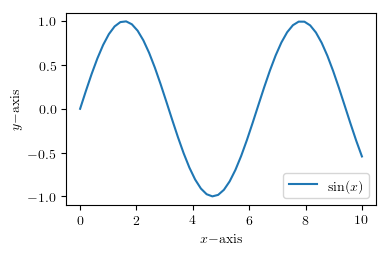
\includegraphics{myplot.pdf}
\end{center}


\section{Basic pylab interaction}

\begin{pylabblock}
from scipy.integrate import quad
myintegral = quad(lambda x: e**-x**2, 0, inf)[0]
\end{pylabblock}

\[ \int_0^\infty e^{-x^2}\,dx = \pylab{myintegral} \]


\section{An automated derivative and integral table}

\pytex\ allows some amazing document automation, such as this derivative and integral table.  Try typing that by hand, fast!

\begin{sympyblock}[][numbers=left,frame=single,framesep=5mm,label=An Automated Derivative and Integral Table]
from re import sub

var('x')

# Create a list of functions to include in the table
funcs = ['sin(x)', 'cos(x)', 'tan(x)', 
         'sin(x)**2', 'cos(x)**2', 'tan(x)**2', 
         'asin(x)', 'acos(x)', 'atan(x)', 
         'sinh(x)', 'cosh(x)', 'tanh(x)']

print(r'\begin{align*}')

for func in funcs:
    # Put in some vertical space when switching to arc and hyperbolic funcs
    if func == 'asin(x)' or func == 'sinh(x)':
        print(r'&\\')
    myderiv = 'Derivative(' + func + ', x)'
    myint = 'Integral(' + func + ', x)'
    print(latex(eval(myderiv)) + '&=' +
            latex(eval(myderiv + '.doit()')) + r'\quad & \quad')
    print(latex(eval(myint)) + '&=' +
            latex(eval(myint+'.doit()')) + r'\\')
print(r'\end{align*}')
\end{sympyblock}

\printpythontex


\section{Step-by-step solutions}

Using SymPy, it is possible to typeset step-by-step solutions.  In this particular case, we also use the \verb|mdframed| package to place a colored background behind our code.

\begin{mdframed}[linecolor=Green,innerrightmargin=30pt,innerleftmargin=30pt,leftmargin=-30pt,rightmargin=-30pt,backgroundcolor=Black!5,skipabove=10pt,skipbelow=10pt,roundcorner=5pt,frametitle={Step-by-Step Integral Evaluation},frametitlealignment=\center,splitbottomskip=6pt,splittopskip=12pt]
\begin{sympyblock}[][numbers=left]
x, y, z = symbols('x,y,z')
f = Symbol('f(x,y,z)')

# Define limits of integration
x_llim = 0
x_ulim = 2
y_llim = 0
y_ulim = 3
z_llim = 0
z_ulim = 4

print(r'\begin{align*}')

# Notice how I define f as a symbol, then later as an actual function
left = Integral(f, (x, x_llim, x_ulim), (y, y_llim, y_ulim), (z, z_llim, z_ulim))
f = x*y + y*sin(z) + cos(x+y)
right = Integral(f, (x, x_llim, x_ulim), (y, y_llim, y_ulim), (z, z_llim, z_ulim))
print(latex(left) + '&=' + latex(right) + r'\\')

# For each step, I move limits from an outer integral to an inner, evaluated 
# integral until the outer integral is no longer needed
right = Integral(Integral(f, (z, z_llim, z_ulim)).doit(), (x, x_llim, x_ulim),
                 (y, y_llim, y_ulim))
print('&=' + latex(right) + r'\\')

right = Integral(Integral(f, (z, z_llim, z_ulim), (y, y_llim, y_ulim)).doit(),
                 (x, x_llim, x_ulim))
print('&=' + latex(right) + r'\\')

right = Integral(f, (z, z_llim, z_ulim), (y, y_llim, y_ulim), 
                 (x, x_llim, x_ulim)).doit()
print('&=' + latex(right) + r'\\')

print('&=' + latex(N(right)) + r'\\')

print(r'\end{align*}')
\end{sympyblock}
\end{mdframed}

\printpythontex


\section{Including stderr}

\pytex\ allows code to be typset next to the stderr it produces.  This requires the package option \verb|makestderr|.

\begin{pyblock}[errorsession][numbers=left]
x = 123
y = 345
z = x + y +
\end{pyblock}

This code causes a syntax error:

\stderrpythontex[verbatim][frame=single]

The package option \verb|stderrfilename| allows the file name that appears in the error message to be customized.




\end{document}
